This chapter provides an overview of future work areas for further research. \cref{sec:zero_shot} includes ideas for improving the state-of-the-art. We also propose four ideas for synthetic dataset generation (\cref{sec:synthetic_dataset}). Finally, we include some ideas for extending current datasets to be multilingual (\cref{sec:multilingual_datasets}).

\section{Zero-shot Experiments} \label{sec:zero_shot}

Future work could improve results on Winoground and VSR by training and fine-tuning better VLMs. We could also check if there is any new appropriate dataset to evaluate models. New SOTA systems might appear in the future and we could check if they improve results. We could conduct an in-depth quantitative and qualitative analysis of the results to explain the limitations of different types of VLMs.

In the future, we might investigate the use of \textbf{multi-tasking} and \textbf{multi-sourcing} to improve generalization properties. In a multi-task training paradigm, the model is forced to learn more than one task simultaneously, therefore improving its generalization capabilities. We could investigate multi-task settings to combine the verbalized dataset, the images produced by the generative VLMs, as well as traditional training data to obtain spatial-aware language models.

We could also improve \textbf{zero-shot} and \textbf{few-shot} generalization of VLM models to obtain effective models in small data regimes of the spatial reasoning domain. Thus eliminating the necessity of explicitly annotating big quantities of spatial relations.

\section{Synthetic Dataset Creation} \label{sec:synthetic_dataset}

As to avoid the scarcity of multimodal datasets that explicitly describe spatial relations, we propose to automatically construct synthetic datasets. We could then use them to train existing language models in a self-supervised way, with the final aim of obtaining spatially grounded language models. We propose four options that could be combined to produce the synthetic datasets: explicit verbalization (\ref{sec:explicit_verbalization}), text-to-image (\ref{sec:text-to-image}), image-to-image (\ref{sec:image-to-image}) and image captioning and retrieval (\ref{sec:image_captioning_retrieval}).

\subsection{Explicit Verbalization} \label{sec:explicit_verbalization}

Explicit verbalization could be used to perform synthetic data generation to learn spatial grounding. Explicit verbalization can be extracted directly from the image. Given an image in an existing dataset that contains spatial relations (MS COCO), we propose to use an object detector to identify the entities in the images. Then, we could create hand-designed verbalization templates to automatically generate textual descriptions of the spatial relations among them.

Finally, we could train existing LMs in a self-supervised way using the synthetic dataset. We could test various methods for verbalization to know which is the right way to verbalize spatial information for effective spatial grounding. Then, we can test if we can improve the state-of-the-art of vision and language models in tasks that require spatial reasoning.

\subsection{Text-to-Image Generation} \label{sec:text-to-image}

Large generative \textbf{text-to-image diffusion models}, like DALLE-2 \cite{ramesh2022hierarchical} and IMAGEN \cite{saharia2022photorealistic}, are able to generate stunning images. They are known to possess some visual-reasoning skills \cite{cho2022dall}. However, in our work, we have seen that Stable Diffusion makes many mistakes when generating images, which require compositional reasoning.

A recent work \cite{liu2022compositional} has also shown that these models \textbf{struggle to understand the composition of some concepts}, such as confusing the attributes and relations of different objects. They propose a new method, where an image is generated by composing a set of diffusion models, with each of them modelling a certain component of the image. Yet, this approach requires modifying the input prompts and is limited only to conjunction (and) and negation (not). Winoground examples are more complex, and can not be simplified to a conjunction of objects.

Another work \cite{anonymous2023trainingfree} proposes manipulating cross-attention representations to address three challenging phenomena in Stable Diffusion \cite{rombach2021highresolution}: \textbf{attribute leakage}, \textbf{interchanged attributes} and \textbf{missing objects} (see \cref{fig:training-free}). They achieve better compositional skills in qualitative and quantitative results, leading to a very significant 5-8\% advantage in head-to-head user comparison studies. Many of the problems when generating Winoground images are of this type. Therefore, this might improve results when generating Winoground images.

\begin{figure}[ht]
    \centering
    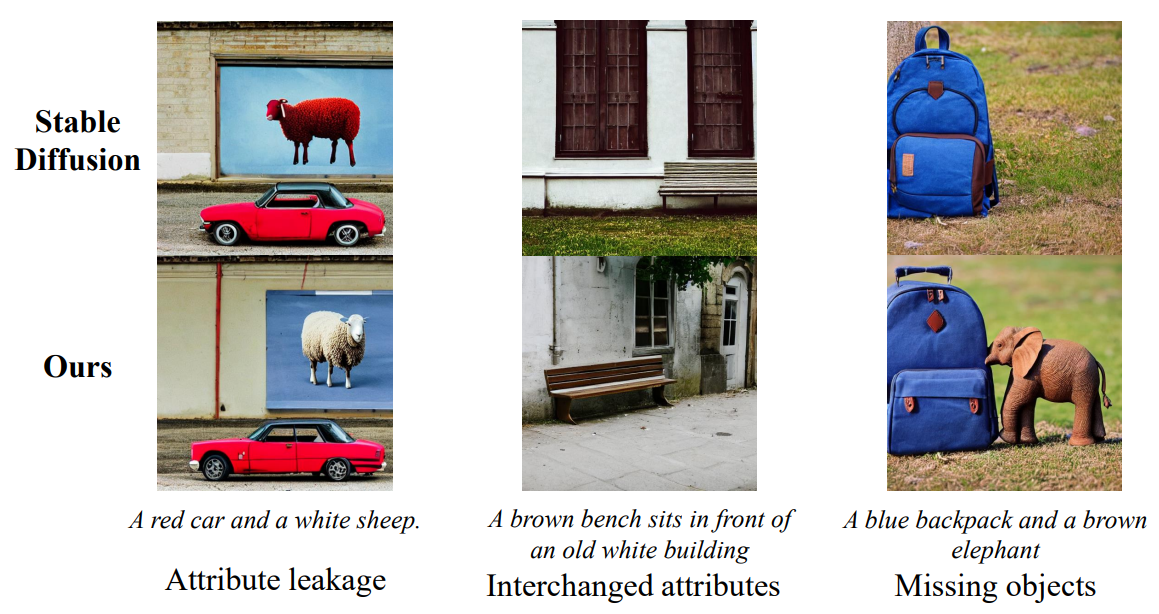
\includegraphics[width=\linewidth]{images/future/training-free.png}
    \caption{Three challenging phenomena in the compositional generation. Attribute leakage: The attribute of one object appears in another object. Interchanged attributes: the attributes of two or more objects are interchanged. Missing objects: one or more objects are missing.}
    \label{fig:training-free}
\end{figure}

\subsection{Image-to-Image Generation} \label{sec:image-to-image}

Apart from text-to-image generation, diffusion models can also be used for image-to-image generation. Stable Diffusion \cite{rombach2021highresolution} could be used to generate new images as a data augmentation technique. For example, multiple image \textbf{variations} can be generated from an input image, to get similar images that still match the original caption. We could also change the caption if we are interested in getting similar images with different objects. 

The problem with variations is that even a small change in the text prompt can lead to a completely different outcome. Usually, we only want to edit a small part of an image, without affecting the rest of the image. State-of-the-art methods solve this with \textbf{in-painting}, by using a spatial mask to localize the edit, leaving the rest of the image untouched.

The drawback of this approach is that spatial masks have to be specifically crafted for each edit. A solution for this is to do image editing only using text prompts, that is, \textbf{prompt-to-prompt} editing \cite{hertz2022prompt}. This technique allows many types of edits such as localized editing by replacing a word, and global editing by adding a specification and controlling the extent to which a word is reflected in the image (\cref{fig:prompt-to-prompt}).

\begin{figure}[ht]
    \centering
    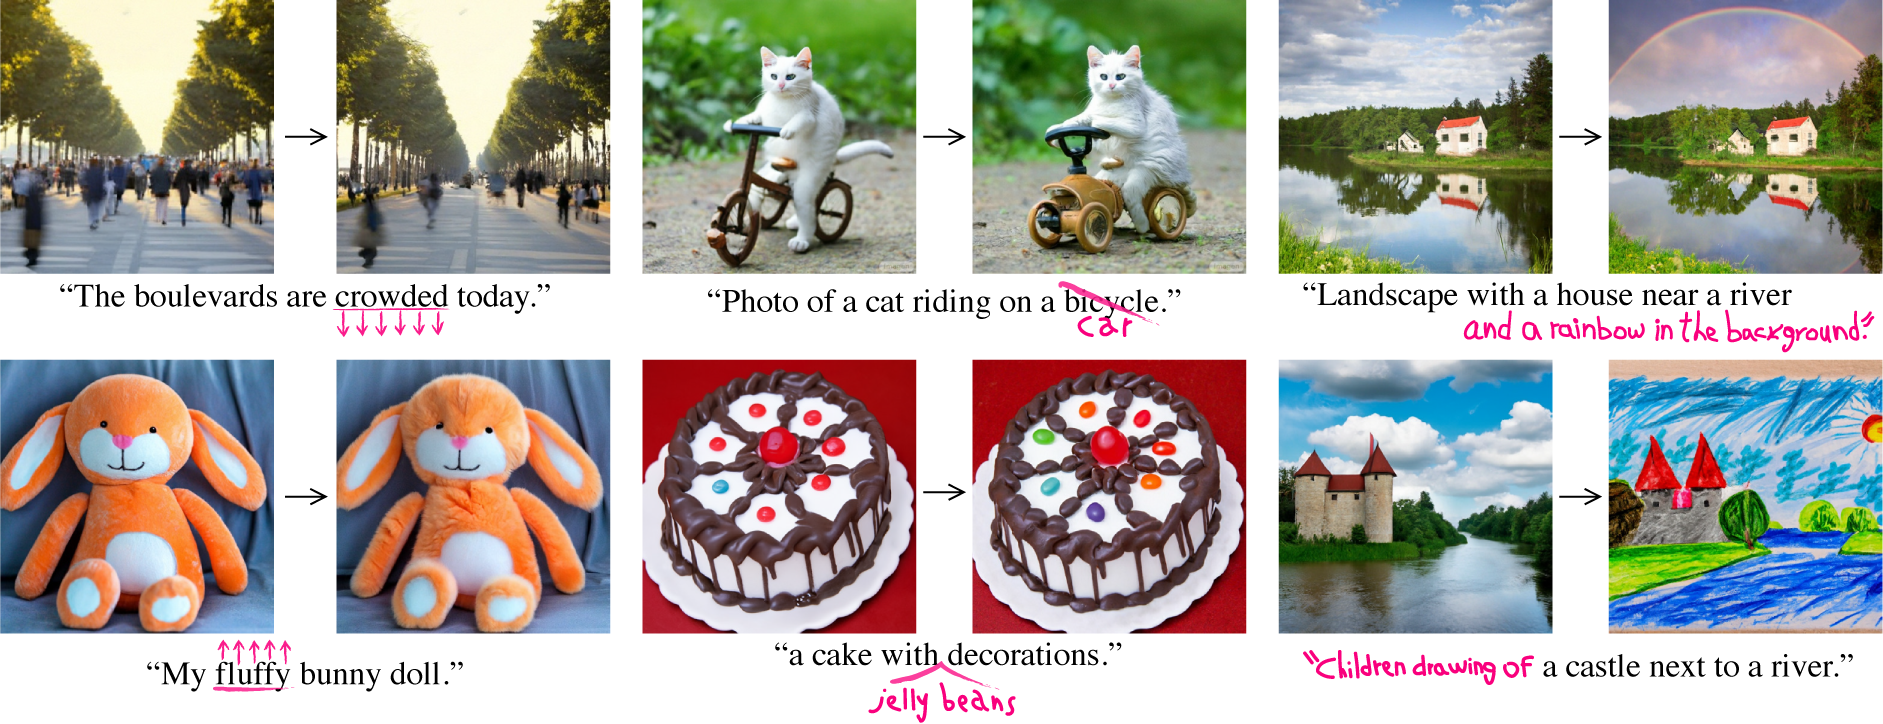
\includegraphics[width=\linewidth]{images/future/prompt-to-prompt.png}
    \caption{Prompt-to-Prompt editing operations: tuning the level of influence of an adjective word (left), making a local modification in the image by replacing or adding a word (middle), or specifying a global modification (right).}
    \label{fig:prompt-to-prompt}
\end{figure}

\subsection{Image Captioning and Retrieval} \label{sec:image_captioning_retrieval}

In this work, we have seen that generating synthetic captions can be a good approach to automatically describe images at a large scale. We have also seen that image retrieval can be used to retrieve images from a huge dataset given a caption or an image. In the future, captioning could be paired with image retrieval to create a synthetic dataset. This way, we can retrieve images that we are interested in, and generate good captions for them.

LAION-COCO\footnote{\url{https://laion.ai/blog/laion-coco/}} is a new dataset that follows a similar approach. It is the world’s largest dataset of this type, with 600M generated high-quality captions for public images from LAION2B-EN \cite{schuhmann2022laionb}. LAION5B already has natural captions, but these captions are generally not very good and could be completed by synthetic ones. These captions could be used to train VLMs to investigate how they impact the performance of models.

The model used to generate captions is the same one that we used (BLIP L/16), but they do some extra steps to increase caption quality. First, they generate 40 captions at a time, which are later ranked using CLIP L/14 to select the best 5 captions. Then, those captions are ranked using CLIP RN50x64 to select the best one. Finally, a small fine-tuned T0 model is used to repair the grammar and punctuation errors in the texts.

They evaluated these captions by asking human evaluators to guess whether it corresponds to a human or an AI model. They also asked them to rate the quality on a scale from 0 (bad) to 5 (good). They presented each evaluator with 200 samples, that contained 100 AI-generated and 100 human-written MS COCO captions. They conclude that caption quality is on average pretty close to the human-written captions of MS COCO. Filters could be further improved by rating more images by humans and removing low-score images.

Image captioning could also be used to extend current datasets to other languages. Multilingual VLMs could be used to caption the same image and get captions in many languages. A recent dataset called Crossmodal-3600 aims to evaluate multilingual image captioning \cite{thapliyal2022crossmodal}. It contains a geographically-diverse set of 3600 images annotated with human-generated reference captions in 36 languages. This dataset could be used to evaluate multilingual models and decide if they are good enough to generate synthetic datasets.

\section{Multilingual Datasets} \label{sec:multilingual_datasets}

Another direction is extending Winoground and VSR to cover more languages and cultures and testing multilingual VLMs. There are already some multilingual visual reasoning datasets. MaRVL (Multicultural Reasoning over Vision and Language) \cite{liu-etal-2021-visually} consists of discriminating whether each grounded statement about a pair of images is true or false. It focuses on a typologically diverse set of languages, Indonesian, Mandarin Chinese, Swahili, Tamil, and Turkish. IGLUE (Image-Grounded Language Understanding Evaluation) \cite{bugliarello2022iglue} brings together visual question answering, cross-modal retrieval, grounded reasoning, and grounded entailment tasks across 20 diverse languages.

Winoground is English-only and translation to other languages may be difficult. The key aspect of Winoground is that both captions contain the same words. Translating to other languages and maintaining this characteristic might be very difficult, and probably impossible in some examples. Moreover, expert translation is time-consuming and that limits the size of the translated datasets. 

VSR seems to be easier to translate because it has no restrictions about the used words. However, spatial relations can be very different across languages. Some relations that are common in English might not exist in other languages and vice versa. In addition, word order is different from English in many languages, and that hinders template-based caption creation.

Apart from evaluation datasets, good pretraining multilingual datasets are needed to create multilingual VLMs. For example, LAION-5B \cite{schuhmann2022laionb} dataset was automatically collected from the web. It has two multilingual subsets, one with an unknown language (LAION1B-nolang) and the other one with a known (LAION2B-multi). Recently, a new dataset called LAION-translated\footnote{\url{https://laion.ai/blog/laion-translated/}} was released based on the previous ones. Every caption of the original datasets was translated to English with Facebook’s M2M100 1.2B model. These captions can be used to train a multilingual VLM using aligned pairs.

